\chapter{Entscheidungen und Optimierung}

\nextlecture{10. 04, 2025}[Präferenrelationen: Beispiele, Rationalität, Monotonie \& Indifferenzkurven]
\section{Präferenzen}
In der mikroökonomischen Theorie bilden die \emph{Präferenzen} eines Individuums die Grundlage für die Analyse von Konsumentscheidungen.
Präferenzen beschreiben, wie ein Individuum verschiedene Alternativen bewertet und miteinander vergleicht.

\begin{definition}[Güterbündel] \index{Güterbündel}
	Ein Vektor $x = (x_1,\dotsc,x_n)$, indem $x_i$ die Mengeangabe des Guts $i$ beschreibt, heißt \defemph{Güterbündel}
\end{definition}
\begin{remark}
	Theoretisch können unserer Güterbündel \enquote{unendlich} fortgesetzt werden, indem wir die restlichen Einträge einfach $0$ setzen, da diese Güter dann keine wirkliche Rolle spielen.
\end{remark}
\begin{example}
	Betrachten wir einen Konsumenten, der sich zwischen zwei Güterbündeln entscheiden muss:
	\begin{itemize}
		\item $x = (2 \text{ Äpfel}, 3 \text{ Birnen})$
		\item $y = (1 \text{ Apfel}, 4 \text{ Birnen})$
	\end{itemize}
	Der Konsument kann entweder $x$ gegenüber $y$ bevorzugen, $y$ gegenüber $x$ bevorzugen oder beide als gleichwertig betrachten. Um diese Vorlieben systematisch zu modellieren, verwenden wir eine \textit{Präferenzrelation}.
\end{example}

\begin{definition}[Präferenzrelation]
	Sei $X$ die Menge aller möglichen Güterbündel.
	Ein \defemph{Präferenzrelation} $\succeq$ \glsadd{präferenz} auf $X$ ordnet jedem Paar von Güterbündeln $(x, y) \in X \times X$ eine Aussage darüber zu, ob das Güterbündel $x$ mindestens ebenso gut ist wie das Güterbündel $y$.
\end{definition}
Eine Präferenzrelation ist also wie eine persönliche Rangliste oder ein Vergleichssystem. Sie hilft uns zu verstehen, wie jemand Entscheidungen trifft, wenn er zwischen verschiedenen Optionen wählen kann.
\begin{notation}
	Zusätzlich einigen wir uns auf das Folgende:
	\begin{itemize}
		\item $x \succ y \ \Leftrightarrow\  x \succeq y$ und nicht $y \succeq x$ (strikte Präferenz) \glsadd{strikte-präferenz}
		\item $x \sim y \ \Leftrightarrow\  x \succeq y$ und $y \succeq x$ (Indifferenz) \glsadd{indifferenz}
	\end{itemize}
\end{notation}

Wir können uns diese Notation ähnlich vorstellen, wie bei dem Vergleich von Zahlen. Das heißt, beispielsweise, wenn wir sagen wollen, dass $9 > 8$ ist, können wir auch sagen, dass $9 \ge 8$ und $8 \ngeq 9$ ist.
Wenn $9\ge 9$ und $9 \le 9$ gilt, dann schreiben wir $9=9$, wir sind sozusagen indifferent.
Die Eigenschaften der $\ge$-Relation erfüllt zwei wichtige Annahmen, ohne diese unsere Notation überhaupt erst sinnvoll bzw. möglich wird.
\begin{definition}
	Eine Präferenzrelation wird als \defemph{rational}\index{Präferenz!rational} bezeichnet, wenn sie folgende Eigenschaften erfüllt:
	\begin{itemize}
		\item \defemph{Vollständigkeit:} Für alle $x, y \in X$ gilt: $x \succeq y$ oder $y \succeq x$ (oder beides). \index{Präferenz!Vollständigkeit}
		\item \defemph{Transitivität:} Für alle $x, y, z \in X$ gilt: Wenn $x \succeq y$ und $y \succeq z$, dann auch $x \succeq z$. \index{Präferenz!Transititvität}
	\end{itemize}
\end{definition}

Die Eigenschaft der \textbf{Vollständigkeit} bedeutet, dass eine Person in der Lage ist, jedes beliebige Paar von Güterbündeln miteinander zu vergleichen. Für alle denkbaren Kombinationen aus zwei Alternativen gilt:
\begin{itemize}
	\item Entweder wird das erste Güterbündel dem zweiten vorgezogen,
	\item das zweite dem ersten vorgezogen oder
	\item beide werden als gleich gut empfunden.
\end{itemize}


Die Eigenschaft der \textbf{Transitivität} sorgt dafür, dass Präferenzen widerspruchsfrei sind. Sie besagt:
\begin{quote}
	Wenn ein Individuum Güterbündel $A$ gegenüber $B$ bevorzugt ($A \succeq B$) und $B$ gegenüber $C$ bevorzugt ($B \succeq C$), dann sollte es auch $A$ gegenüber $C$ bevorzugen ($A \succeq C$).
\end{quote}

\begin{example}
	Sollte gelten, dass
	\begin{itemize}
		\item $A$ (2 Äpfel, 3 Birnen) wird gegenüber $B$ (1 Apfel, 4 Birnen) bevorzugt.
		\item $B$ wird gegenüber $C$ (1 Apfel, 2 Birnen) bevorzugt.
	\end{itemize}
	Dann sollte auch $A$ gegenüber $C$ bevorzugt werden.
\end{example}

Ohne Transitivität wären Präferenzen widersprüchlich. Es könnte vorkommen, dass eine Person $A$ gegenüber $B$ bevorzugt, $B$ gegenüber $C$ und dennoch $C$ gegenüber $A$. Solche Zyklen machen Vorhersagen über Entscheidungen unmöglich und führen zu logischen Problemen bei der Modellierung von Konsumverhalten.
\begin{remark}
	Bei der Präferenzaggregation, kann es öfters zu solchen Problemen kommen, da Präferenzen von verschiedenen Individueen unterschiedlich sind.
\end{remark}
Wir können einige hilfreiche Schlussfolgerungen aus Präferenzrelationen herleiten.
\begin{proposition}
	Sei $\succeq$ eine Präferenzrelation auf einer Menge von Güterbündeln $X$, die \textbf{vollständig} und \textbf{transitiv} ist. Dann gelten für alle $x, y, z \in X$ folgende Eigenschaften:
	\begin{enumerate}
		\item $x \sim z$, wenn $x \sim y$ und $y \sim z$.
		\item $x \succ z$, wenn $x \succ y$ und $y \succ z$.
		\item $x \succ z$, wenn $x \succ y$ und $y \succeq z$.
		\item $x \succ z$, wenn $x \succeq y$ und $y \succ z$.
		\item $x \sim x$ (Reflexivität der Indifferenzrelation).
	\end{enumerate}
\end{proposition}

\begin{proof}
	Da $\succeq$ vollständig und transitiv ist, gelten folgende Schlussfolgerungen:

	\begin{enumerate}
		\item
		      Aus $x \sim y$ und $y \sim z$ folgt per Definition: $x \succeq y$, $y \succeq x$, $y \succeq z$ und $z \succeq y$.
		      Durch Transitivität gilt dann:
		      \begin{align*}
			      x \succeq z             & \text{ (da } x \succeq y \text{ und } y \succeq z) \\
			      \text{und } z \succeq x & \text{ (da } z \succeq y \text{ und } y \succeq x)
		      \end{align*}
		      Damit ist $x \sim z$.

		\item
		      Aus $x \succ y$ und $y \succ z$ folgt per Definition:
		      \begin{align*}
			      x \succeq y \text{ und } y \nsucceq x \\
			      y \succeq z \text{ und } z \nsucceq y
		      \end{align*}
		      Wegen der Transitivität gilt $x \succeq z$.
		      Nun bleibt zu zeigen, dass $z \nsucceq x$.
		      Angenommen, $z \succeq x$ gilt. Dann würde zusammen mit $x \succeq y$ und $y \succeq z$ durch Transitivität $z \succeq y$ und $y \succeq x$ implizieren, was mit den Annahmen $x \succ y$ und $y \succ z$ einen Widerspruch ergibt.
		      Also gilt $x \succ z$.

		\item
		      Aus $x \succ y$ ($x \succeq y$, $y \nsucceq x$) und $y \succeq z$ folgt durch Transitivität $x \succeq z$.
		      Angenommen, $z \succeq x$ gilt. Dann ergibt sich per Transitivität $z \succeq y$, was mit $x \succ y$ (also $x \succeq y$, $y \nsucceq x$) einen Widerspruch ergibt.
		      Also gilt $x \succ z$.

		\item  Analog zu (3):
		      Aus $x \succeq y$ und $y \succ z$ folgt $x \succeq z$.
		      Angenommen, $z \succeq x$ gilt. Dann folgt $z \succeq y$ per Transitivität (da $z \succeq x$ und $x \succeq y$), was mit $y \succ z$ (also $y \succeq z$,  $z \nsucceq y$) einen Widerspruch ergibt.
		      Also gilt $x \succ z$.

		\item Die Eigenschaft $x \sim x$ ist unmittelbar gegeben, da jede Präferenzrelation per Definition reflexiv bezüglich Indifferenz ist: $x \succeq x$ und $x \succeq x$ implizieren $x \sim x$.
	\end{enumerate}

\end{proof}
\begin{remark}
	Die letzte Eigenschaft, also die \emph{Reflexivität} ist in unserer Definition nicht gegeben, das heißt es ist formal nötig, dass wir auch $x \succeq x$ angeben müssen für alle $x \in X$.
	Oft wird dies aber aus \enquote{Faulheit} bzw. Klarheit weggelassen.
\end{remark}

Prinzipell ist es möglich, dass Konsumten Güterbündel bevorzugen, die von allem weniger Mengen haben, wir gehen in den meisten Fällen jedoch davon aus, dass Konsumenten Güterbündel mit generell mehr Mengen bevorzugen.

\begin{definition}[monotone Präferenz]
	Sei $X$ die Menge aller möglichen Güterbündel und $\succeq$ eine Präferenzrelation auf $X$.
	Die Präferenzrelation $\succeq$ heißt \textbf{monoton}\index{Präferenz!monoton}, wenn gilt:

	\begin{quote}
		Für alle $x, y \in X$: Wenn $x_i \geq y_i$ für alle Güter $i$ und $x \neq y$, dann gilt $x \succ y$.
	\end{quote}

\end{definition}
\noindent Das bedeutet:
\begin{itemize}
	\item Ein Konsument bevorzugt ein Güterbündel gegenüber einem anderen, wenn es von mindestens einem Gut mehr enthält, aber von keinem weniger.
	\item Mehr von einem Gut (bei gleichbleibender Menge der anderen Güter) macht ein Güterbündel strikt besser.
\end{itemize}

\begin{remark}
	Diese Annahme spiegelt wieder, dass „mehr ist besser“ gilt — zumindest solange keine Sättigung erreicht ist und keine negativen Güter (wie Müll oder Krankheit) berücksichtigt werden.
\end{remark}


\begin{example}
	Betrachten wir die zwei Güterbündel:
	\begin{itemize}
		\item $x=(1,2,3,4)$
		\item $y=(2,3,4,5)$
	\end{itemize}
	Eine Präferenz ist monoton in diesem Fall, wenn $y \succeq x$ gilt.
\end{example}


\section{Nutzen}

Eine Nutzenfunktion ist eine reellwertige Funktion $U: X \rightarrow \mathbb{R}$, die jedem möglichen Konsumbündel $(x_1, x_2, ..., x_n)$ im Güterraum $X$ einen numerischen Wert zuordnet, der das relative Maß an Zufriedenheit oder Nutzen widerspiegelt, das der Konsument aus dem Konsum dieses Bündels zieht.

\begin{definition} \label{def:nutzenfunktion}
	Sei $X \subseteq \mathbb{R}^n_+$ der $n$-dimensionale Güterraum. Eine \defemph{Nutzenfunktion} ist eine Abbildung $U: X \rightarrow \Real$, sodass für zwei Güterbündel $A, B \in X$ gilt:
	\begin{itemize}
		\item $A \succsim B \iff U(A) \ge U(B)$
		\item $A \sim B \iff U(A) = U(B)$
	\end{itemize}
\end{definition}

Mit der Nutzenfunktion vergeben wir für unser Rankingsystem (also der Präferenz) sozusagen Punkte.
Das heißt, wenn wir Schokolade schwach gegenüber Gummibärchen bevorzugen und Gummibärchen eine Wertung von $9$ erhalten, dann muss Schokolade ebenfalls eine Wertung von mindestens $9$ erhalten.
Es spielt dabei keine Rolle, wie die Abstände sind, solange es mit der Präferenz einher geht.


\subsection{Indifferenzkurven}
Eine \emph{Indifferenzkurve} ist die Menge aller Konsumbündel aus einem Güterraum, die dem Konsumenten denselben Nutzen stiften.

\begin{definition}[Indifferenzkurve]
	Gegeben eine Nutzenfunktion \( u: X \rightarrow \mathbb{R} \), mit \( X \subseteq \mathbb{R}_+^n \)\footnote{Wir beschränken uns meist auf den Fall $\Real^2$, da wir dort die Indifferenzkurven einfach zeichnen können.} als Güterraum, ist die \defemph{Indifferenzkurve} \index{Indifferenzkurve} zum Nutzeniveau \( \bar{u} \) definiert als:
	\[
		I_{\bar{u}} = \left\{ \mathbf{x} \in X \,\bigg|\, u(\mathbf{x}) = \bar{u} \right\}
	\]
\end{definition}

Die Idee besteht nun darin, Präferenzen grafisch darzustellen, indem wir
Kurven durch die Bündel zeichnen, zwischen denen der Konsument
indifferent\footnote{Betrachten wir die Definition einer Höhenlinie, sehen wir, dass diese im wesentlich - mit anderen Bezeichnungen - gleich sind. Diese werden auch analog bestimmt.} ist – das heißt, die er als gleichwertig erachtet


\begin{example}
	Betrachten wir die Nutzenfunktion $u(x,y) = x\cdot y$. Die Indifferenzkurve sieht dann wie folgt aus:
	\begin{center}
		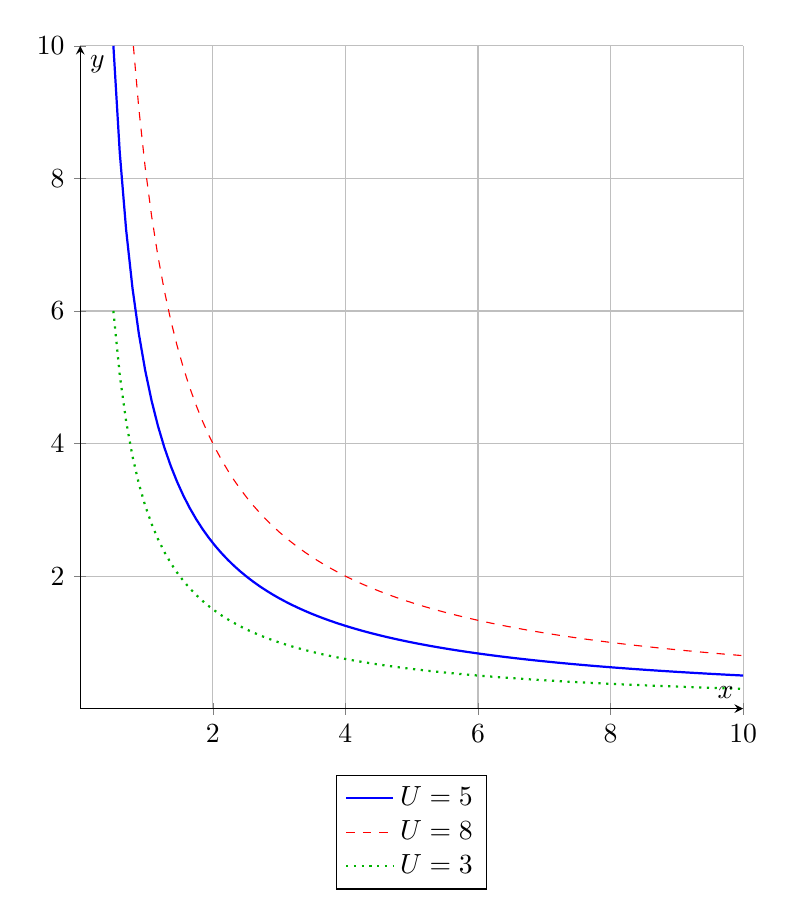
\begin{tikzpicture}
			\begin{axis}[
					axis lines = middle,
					xlabel={$x$},
					ylabel={$y$},
					xmin=0, xmax=10,
					ymin=0, ymax=10,
					domain=0.5:10,
					samples=100,
					width=10cm,
					height=10cm,
					grid=both,
					legend style={at={(0.5,-0.1)},anchor=north},
				]

				% Indifferenzkurven für verschiedene Nutzen-Niveaus
				\addplot [blue, thick] {5/x};
				\addlegendentry{$U=5$}

				\addplot [red, dashed] {8/x};
				\addlegendentry{$U=8$}

				\addplot [green!70!black, dotted, thick] {3/x};
				\addlegendentry{$U=3$}

			\end{axis}
		\end{tikzpicture}
	\end{center}
	Die Grafik erhalten wir, indem wir unsere Funktion $u(x,y)$ gleich einem konstanten Wert setzen.
	Allgemein für die Funktion $u(x,y) = x\cdot y$ erhalten wir dann:
	\begin{align*}
		u(x,y) = x \cdot y = c \implies y = \frac{c}{x}
		.\end{align*}
	Wir erkennen hier also die Ähnlichkeit zur Funktion $\frac{1}{x}$.
\end{example}

\begin{lemma} \label{lem:indifferenzkurve}
	Sei $U: \mathbb{R}_{+}^2 \rightarrow \mathbb{R}$ eine stetige, streng monoton wachsende und quasikonvexe Nutzenfunktion, die ein vollständiges und transitives Präferenzsystem auf $\mathbb{R}_{+}^2$ repräsentiert.
	Für alle $c_1, c_2 \in \mathbb{R}$ mit $c_1 \neq c_2$ gilt:
	\begin{enumerate}
		\item $I(c_1) \cap I(c_2) = \varnothing$
		\item Für alle $(x_1, y_1), (x_2, y_2) \in \mathbb{R}_{+}^2$ gilt: $U(x_2, y_2) > U(x_1, y_1) \iff (x_2, y_2)$ liegt auf Indifferenzkurve weiter vom Ursprung entfernt als $(x_1, y_1)$.

	\end{enumerate}
\end{lemma}

\begin{proof}
	Wir zeigen beide Aussagen getrennt.

	\begin{enumerate}
		\item
		      Angenommen, es existiert ein Punkt $(x^*, y^*) \in \mathbb{R}_{+}^2$ mit
		      \[
			      (x^*, y^*) \in I(c_1) \cap I(c_2)
		      \]
		      Dann gilt per Definition:
		      \[
			      U(x^*, y^*) = c_1 \quad \text{und} \quad U(x^*, y^*) = c_2
		      \]
		      Daraus folgt unmittelbar:
		      \[
			      c_1 = c_2
		      \]
		      Dies widerspricht der Voraussetzung $c_1 \neq c_2$.
		      Also ist die Annahme falsch und es gilt:
		      \[
			      I(c_1) \cap I(c_2) = \varnothing
		      \]

		\item	Seien zwei Güterbündel $(x_1, y_1), (x_2, y_2) \in \mathbb{R}_{+}^2$ gegeben.

		      Da $U$ streng monoton ist, gilt:
		      \begin{itemize}
			      \item Wenn $(x_2, y_2)$ gegenüber $(x_1, y_1)$ bei mindestens einem Gut größer ist und beim anderen mindestens gleich, dann ist
			            \[
				            U(x_2, y_2) > U(x_1, y_1)
			            \]
			      \item In diesem Fall liegt $(x_2, y_2)$ auf einer Indifferenzkurve mit höherem Nutzenniveau.
		      \end{itemize}
		      Da Indifferenzkurven mit höherem Nutzenniveau (wegen strenger Monotonie) weiter vom Ursprung entfernt liegen müssen (mehr von mindestens einem Gut erhöht den Nutzen und verschiebt die Kurve nach außen), folgt die Äquivalenz.

	\end{enumerate}
\end{proof}

Lemma \ref{lem:indifferenzkurve} sagt aus, dass sich zwei Indifferenzkurven nicht schneiden können. Dies ergibt auch Sinn, mathematisch kann eine Indifferenzkurve auch als Höhenlinie aufgefasst werden.
Also eine Höhenlinie, wie auf einer Landkarte. Würden sich also zwei dieser Linien schneiden, dann müsste ein Punkt zwei verschiedenen Höhen gleichzeitig haben.
Genauso hat jeder Punkt im "Güterraum" (die verschiedenen Kombinationen von Dingen) ein bestimmtes Zufriedenheitslevel, und kann daher nicht auf zwei verschiedenen Indifferenzkurven mit unterschiedlichem Nutzen liegen.
Die zweite Ausssage beschreibt das die Indifferenzkurve, die am weitesten vom Ursprung weg ist, die \enquote{Beste} für einen ist.
Da jede Indifferenzkurve alle Kombinationen mit dem gleichen Zufriedenheitslevel verbindet, müssen die Kurven, die weiter vom Ursprung entfernt liegen, Kombinationen mit mehr von den Gütern darstellen und dir daher ein höheres Level an Zufriedenheit (höheren Nutzen) bringen.

\begin{remark}
	Ist die Monotonieannahme einer Präferenz erfüllt, so können Indifferenzkurven keine Flächen sein. Auch können diese keine positive Steigung haben, da sonst die Güter weiter rechts größere Mengenangaben haben, sodass diese strikt den anderen Gütern bevorzugt werden.
\end{remark}

\subsection{Nutzenfunktion}

\nextlecture{12. 04, 2025}[Nutzenfunktionen, monotone Tranfsformation]

Wir haben in Definition \ref{def:nutzenfunktion} bereits gelernt, was eine Nutzenfunktion ist.
Diese Definition sagt indirekt auch, dass verschiedene Nutzenfunktionen gleiche Präferenzen beschreiben können. Es ist natürlich, dass wir eine möglichst einfache Nutzenfunktion zu unserer Präferenz erhalten möchten.

\begin{theorem}[Monotone Transformation] \index{Nutzenfunktion!monotone Transformation}
	Sei \( u: X \to \mathbb{R} \) eine Nutzenfunktion, die eine Präferenzrelation \( \succeq \) repräsentiert. Dann repräsentiert auch jede streng monoton wachsende Transformation \( f: \mathbb{R} \to \mathbb{R} \) der Nutzenfunktion, also \( v = f \circ u \), dieselbe Präferenzrelation.

	\[
		u(\mathbf{x}) \geq u(\mathbf{y}) \iff v(\mathbf{x}) \geq v(\mathbf{y}) \quad \text{für alle } \mathbf{x}, \mathbf{y} \in X
	\]
\end{theorem}

\begin{proof}
	Sei \( f: \mathbb{R} \rightarrow \mathbb{R} \) streng monoton wachsend und \( u: X \rightarrow \mathbb{R} \) eine Nutzenfunktion.

	Definiere \( v(\mathbf{x}) = f(u(\mathbf{x})) \).

	Da \( f \) streng monoton wachsend ist, gilt:

	\[
		u(\mathbf{x}) \geq u(\mathbf{y}) \iff f(u(\mathbf{x})) \geq f(u(\mathbf{y}))
	\]

	also:

	\[
		u(\mathbf{x}) \geq u(\mathbf{y}) \iff v(\mathbf{x}) \geq v(\mathbf{y})
	\]

	Daher ordnet \( v \) den Güterbündeln dieselben Präferenzen zu wie \( u \).
\end{proof}

\begin{example}
	Betrachten wir die Nutzenfunktion $f(t) = t$. Äquivalent durch monotone Transformation sind:
	\begin{itemize}
		\item $f(t) = t+c$, mit $c \in \Real$
		\item $f(t) = t^3$
		\item $f(t) = \exp(t)$
	\end{itemize}
	Wir können natürlich unendlich weiterer solcher Beispiele konstruieren.
\end{example}

Monotone Transformationen erlauben es uns, die Nutzenfunktion auf verschiedene Arten auszudrücken, ohne die grundlegenden Präferenzen der Person zu verändern.
Die Indifferenzkurven (die Linien gleichen Wohlfühl-Levels) bleiben im Wesentlichen gleich, nur die \enquote{Etiketten} (die Nutzenwerte) ändern sich.

\begin{definition}
	Die \defemph{Grenznutzen} \index{Grenznutzen} der beiden Güter ergeben sich als die partiellen Ableitungen der Nutzenfunktion:

	\[
		\operatorname{MU}_{x_1} = \frac{\partial u(x_1, x_2)}{\partial x_1}, \qquad
		\operatorname{MU}_{x_2} = \frac{\partial u(x_1, x_2)}{\partial x_2}
	\]

\end{definition}
Diese geben an, um wie viel sich der Nutzen ändert, wenn die Menge eines Gutes marginal erhöht wird, während die Menge des anderen konstant bleibt.


\begin{definition}
	Die \defemph{Grenzrate der Substitution (GRS)} \index{Grenzrate der Subsitution} zwischen den Gütern \( x_1 \) und \( x_2 \) gibt das Verhältnis an, in dem der Konsument bereit ist, ein Gut gegen das andere zu tauschen, ohne dabei sein Nutzeniveau zu verändern.
\end{definition}

Formal ergibt sich die GRS aus der Gleichung einer Indifferenzkurve $u(x_1, x_2) = \bar{u}$:

\[
	du = \frac{\partial u}{\partial x_1} dx_1 + \frac{\partial u}{\partial x_2} dx_2 = 0
\]
Daraus folgt:

\[
	\frac{dx_2}{dx_1} = - \frac{\frac{\partial u}{\partial x_1}}{\frac{\partial u}{\partial x_2}} = - \frac{MU_{x_1}}{MU_{x_2}}
\]
Dies ist die \textbf{Grenzrate der Substitution (GRS)} zwischen \( x_1 \) und \( x_2 \).


\begin{center}
	\begin{tikzpicture}[scale=1.2]
		% Achsen
		\draw[->] (0,0) -- (6,0) node[right] {$x_1$};
		\draw[->] (0,0) -- (0,6) node[above] {$x_2$};

		% Indifferenzkurve: u(x1,x2)=3.5 -> x2 = 3.5/x1
		\draw[thick, domain=0.8:5, smooth, variable=\x, blue]
		plot ({\x}, {3.5/\x})
		node[pos=0.95, above] {$u(x_1, x_2) = \bar{u}$};

		% Punkt auf der Indifferenzkurve: (2,1.75)
		\filldraw (2,1.75) circle (2pt) node[above right] {$A$};

		% Tangente an Punkt A mit Steigung -0.875
		\draw[dashed, domain=1:4] plot (\x,{1.75 - 0.875*(\x - 2)});

		% Beschriftung der Tangente
		\node at (4.2, 1.3) {Tangente in $A$};
		\node at (3.9, 0.7) {$\text{Steigung} = -\frac{MU_{x_1}}{MU_{x_2}}$};

		% Hilfslinien zu den Achsen
		\draw[dotted] (2,0) -- (2,1.75);
		\draw[dotted] (0,1.75) -- (2,1.75);
		\node at (2,-0.3) {$x_1^A$};
		\node at (-0.3,1.75) {$x_2^A$};

	\end{tikzpicture}
\end{center}

\begin{example}
	Gegeben sei die Cobb-Douglas Nutzenfunktion:

	\[
		u(x_1, x_2) = x_1^{0.5} \cdot x_2^{0.5}
	\]
	Die Grenznutzen sind die partiellen Ableitungen der Nutzenfunktion:
	\[
		MU_{x_1} = \frac{\partial u(x_1, x_2)}{\partial x_1} = 0.5 \cdot x_1^{-0.5} \cdot x_2^{0.5}
	\]
	\[
		MU_{x_2} = \frac{\partial u(x_1, x_2)}{\partial x_2} = 0.5 \cdot x_1^{0.5} \cdot x_2^{-0.5}
	\]
	Die Grenzrate der Substitution (MRS) ergibt sich als:
	\[
		\operatorname{MRS} = - \frac{MU_{x_1}}{MU_{x_2}} = - \frac{0.5 \cdot x_1^{-0.5} \cdot x_2^{0.5}}{0.5 \cdot x_1^{0.5} \cdot x_2^{-0.5}}
	\]
	Kürzen der 0.5:
	\[
		\operatorname{MRS} = - \frac{x_2}{x_1}
	\]
	Für \( x_1 = 4 \) und \( x_2 = 2 \):

	\[
		\operatorname{MRS} = - \frac{2}{4} = -0.5
	\]
	Das bedeutet, der Konsument ist bereit, 0.5 Einheiten von Gut 2 aufzugeben, um eine Einheit von Gut 1 zu erhalten, wobei der Gesamtnutzen konstant bleibt.
\end{example}



\section{Entscheidungen}

Nachdem wir nun verstehen, wie wir Präferenzen und Nutzenfunktionen modellieren können, möchten wir die Entscheidungen von Konsumenten anhand dieser Untersuchen.
Typischerweise haben Konsumenten nicht unbeschränkten Handlungsfreiraum. Im folgenden werden wir lernen, wie wir dies mathematisch formulieren.

\nextlecture{17. 04, 2025}[Das Problem des Konsumenten und dessen Lösung anhand Cobb-Douglas-Präferenzen]
\subsection{Das Konsumentenproblem}

Als Grundlage für den Konsumenten wählen wir eine Nutzenfunktion, welche wir maximieren möchten.
Die Nebenbedingung stellt dabei seine Einschränkung dar.

\begin{definition}
	Das Budget $m$, des Konsumenten sei gegeben. Die \defemph{Budgetbeschränkung} \index{Budgetbeschränkung} ist gegeben durch:
	\[
		\sum_{i=1}^{n} p_i \cdot x_i  \le m
		.\]
\end{definition}

\begin{example}[Budgetbeschränkung mit zwei Gütern]
	Wir betrachten die Budgetbeschränkung $p_1 x_1 + p_2 x_2 \le  m$. Damit wir diese grafisch darstellen, stellen können, stellen wir diese nach $x_2$ um:
	\[
		x_2 \le  \frac{m-p_1 x_2}{p_2}
		.\]
	Dies liefert uns eine Art Form von $x_2 =f(x_1)$. Daher sieht die Funktion wie in Abbildung \ref{fig:budgetmenge} aus\footnote{Wir können auch einfach die Werte \enquote{raten} und so auf unsere Budgetgerade kommen}.
	\begin{figure}[h]
		\begin{center}

			\begin{tikzpicture}
				% Achsen
				\draw[->] (0,0) -- (6,0) node[right] {$x_1$};
				\draw[->] (0,0) -- (0,4) node[above] {$x_2$};

				% Budgetgerade
				\draw[thick] (0,3.5) -- (5,0);

				% Schraffierte Fläche
				\fill[pattern=north east lines, pattern color=gray] (0,0) -- (0,3.5) -- (5,0) -- cycle;

				% Achsenbeschriftungen
				\node[left] at (0,3.5) {$\frac{m}{p_2}$};
				\node[below] at (5,0) {$\frac{m}{p_1}$};

				% Steigung
				\node at (3,2.1) {$-\frac{p_1}{p_2}$};

				% Ursprung
				\node[below left] at (0,0) {0};
			\end{tikzpicture}

		\end{center}
		\caption{Budgetmenge mit 2 Gütern}
		\label{fig:budgetmenge}
	\end{figure}
	Wenn wir in unserer Budgetbeschränkung \enquote{Gleichheit} vorraussetzen, so erhalten wir keine Fläche, sondern einfach die zu sehende Gerade.
\end{example}

\begin{remark}
	Diese Beschränkung muss nicht die einzige Nebenbedingung sein, oft wird noch ein zusätzliches Limit für ein Gut verlangt, also eine Rationierung. Wie Abbildung \ref{fig:budgetmenge-rationierung}
	\begin{figure}[h]
		\label{fig:budgetmenge-rationierung}
		\centering
		\begin{tikzpicture}
			% Achsen
			\draw[->] (0,0) -- (6,0) node[right] {$x_1$};
			\draw[->] (0,0) -- (0,4) node[above] {$x_2$};

			% Schraffierte Fläche (bis zur Rationierung bei x̂_1)
			\fill[pattern=north east lines] (0,0) -- (0,3.5) -- (3,1.5) -- (3,0) -- cycle;

			% Budgetgerade voll (gestrichelt ab x̂_1)
			\draw[thick] (0,3.5) -- (3,1.5);
			\draw[dashed] (3,1.5) -- (5,0);

			% Achsenbeschriftungen
			\node[left] at (0,3.5) {$\frac{m}{p_2}$};
			\node[below] at (5,0) {$\frac{m}{p_1}$};
			\node[below] at (3,0) {$\hat{x}_1$};

			% Ursprung
			\node[below left] at (0,0) {0};

		\end{tikzpicture}
		\caption{Budgetmenge mit 2 Gütern bei Rationierung}
	\end{figure}
\end{remark}

\begin{construction}[Maximierungsproblem] \label{maximierungsproblem} Wir betrachten eine Nutzenfunktion $u(x_1,\dotsc,x_n)$ und der Budgetbeschränkung $\sum_{k=1}^{n} p_k x_k \le m$. Dann ist das Optimierungsproblem des Konsumenten:
	\[
		\max_{\{x_i\}_{i=1}^{n}} u(x_1,\dotsc,x_n)
		,\]
	unter der Nebenbedingung:
	\begin{align*}
		x_i                    & \ge 0 \forall i \\
		\sum_{i=1}^{n} p_i x_i & \le m
		.\end{align*}
	Damit können wir das Problem bereits lösen mittels Lagrange-Ansatz (oder bei einfachem Problem durch einsetzen der Nebenbedingung). Stellen wir die Lagrange-Funktion auf:
	\[
		\mathcal{L}(x_1,\dotsc,x_n, \lambda) = u(x_1,\dotsc,x_n) + \lambda \left(m- \sum_{i=1}^{n} p_i x_i \right)
		.\]
	Wir berechnen alle notwendigen Bedinungen, also
	\begin{align}
		\frac{\partial \mathcal{L}}{\partial x_i}     & = \frac{\partial u}{\partial x_i} - \lambda p_i \overset{!}{=} 0 \label{eq:lagrange} \\
		\frac{\partial \mathcal{L}}{\partial \lambda} & =  m - \sum_{i=1}^{n} p_i x_i = 0
		.\end{align}
	Aus der Gleichung \eqref{eq:lagrange} folgt, dass \enquote{Gleichungssystem}\footnote{Wir müssen unsere Lösungen natürlich auch in die Nebenbedingung einsetzen.}
	\[
		\frac{\frac{\partial u}{\partial x_i}}{p_i} = \lambda
		.\]
	Im Optimum ist also das Grenznutzen-zu-Preis-Verhältnis für alle Güter gleich.
\end{construction}

\noindent Im Falle von zwei Gütern erhalten wir einen Spezialfall:
\begin{itemize}
	\item Aus der ersten Gleichung erhalten wir:
	      \[
		      \frac{\partial U}{\partial x_1} = \lambda p_1
	      \]
	\item Aus der zweiten Gleichung erhalten wir:
	      \[
		      \frac{\partial U}{\partial x_2} = \lambda p_2
	      \]
\end{itemize}
Nun teilen wir beide Gleichungen:

\[
	\frac{\frac{\partial U}{\partial x_1}}{\frac{\partial U}{\partial x_2}} = \frac{p_1}{p_2}
\]
Das ergibt die Bedingung für das Optimum:

\[
	\frac{\operatorname{MU}_1}{\operatorname{MU}_2} = \frac{p_1}{p_2}
\]
Dies ist gerade die Tangentialbedinung, welche auch in Abbildung \ref{fig:optimallösung-innere} gezeigt ist. Außerdem erinnern wir uns an die Definition der GRS zurück, welche hier auch gegeben ist.

\begin{remark}
	Wir müssen natürlich auch auf Randlösungen prüfen. Die beschrieben Lösung stellt eine innere Lösung dar, wie in Abbildung \ref{fig:optimallösung-innere} grafisch dargestellt.
\end{remark}
\begin{figure}[h!]
	\label{fig:optimallösung-innere}
	\caption{Optimallösung mit zwei Gütern: innere Lösung}
	\begin{center}

		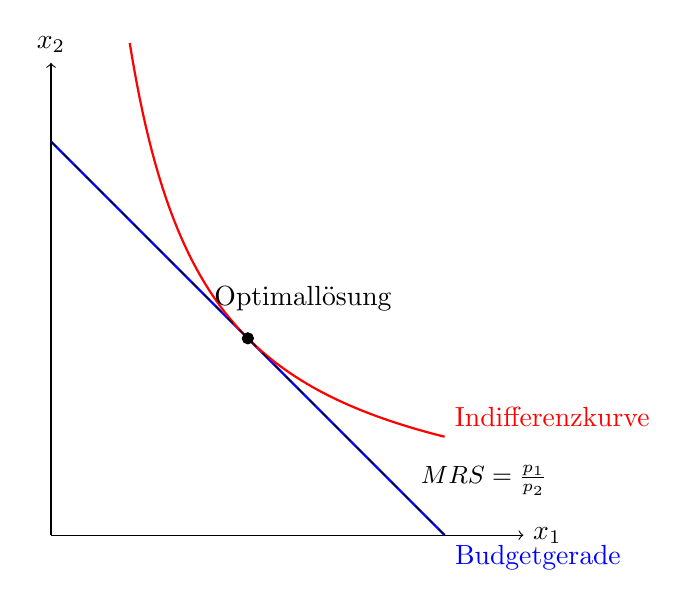
\begin{tikzpicture}
			% Achsen
			\draw[->] (0,0) -- (6,0) node[right] {$x_1$};
			\draw[->] (0,0) -- (0,6) node[above] {$x_2$};

			% Budgetgerade allgemein
			\draw[thick, blue] (0,5) -- (5,0) node[below right] {Budgetgerade};

			% Indifferenzkurve (allgemein gezeichnet, Berührungspunkt bei (2.5,2.5))
			\draw[thick, red, domain=1:5, samples=100] plot(\x, {6.25/(\x)})
			node[above right] {Indifferenzkurve};

			% Tangentialpunkt (Optimallösung)
			\filldraw (2.5,2.5) circle (2pt);
			\node at (3.2,3) {Optimallösung};

			% Tangente an der Indifferenzkurve im Berührungspunkt
			\draw[dashed] (0,5) -- (5,0);

			% Hinweis auf die Bedingung im Tangentialpunkt
			\node at (5.5,0.7) {\small $MRS = \frac{p_1}{p_2}$};

		\end{tikzpicture}

	\end{center}
\end{figure}

\noindent Im folgenden möchten wir ein Beispiel berechnen, dass eine Lösung für eine Klasse von Funktionen liefert, die in der Volkswirtschaftslehre häufig verwendet wird.
\begin{example}[Cobb-Douglas-Präferenzen]
	Wir betrachten die Nutzenfunktion der Konsumentin
	\[
		u(x_1,x_2) = x_1^{\alpha} x_2^{1-\alpha}
	\]
	mit $\alpha \in (0,1)$.
	Dazu berechnen wir zu erst die Grenzrate der Subsitution:
	\begin{align*}
		\operatorname{GRS} & = \frac{\operatorname{MU}_1}{\operatorname{MU}_2} = \frac{\alpha x_1^{\alpha-1}x_2^{1-\alpha}}{(1-\alpha)x_1^{\alpha} x_2^{-\alpha}} \\
		                   & = \frac{\alpha}{1-\alpha} \frac{x_{2}}{x_1}
		.\end{align*}
	Nun liefert uns die Tangentialbedinung $\operatorname{MRS} = \frac{p_1}{p_2}$ in Kombination mit der Budgetbeschränkung $m= p_1x_1+p_2x_2$, unsere möglichen Lösungen:
	\[
		\begin{cases}
			x_1 = \frac{\alpha m }{p_1} \\
			x_2 = \frac{(1-\alpha) m}{p_2}
		\end{cases}
		.\]
	Dies ist hier auch die einige mögliche Lösung, da der Nutzen gleich Null ist, wenn der Konsument eines der Güter
	nicht konsumiert.
	Demnach löst $(x_1,x_2)$ unser Konsumentenproblem.
\end{example}
\begin{remark}
	Ein Konsument mit Cobb-Douglas Präferenzen gibt immer den gleichen
	Anteil seines Budget für jedes der Güter aus! Dies ermöglicht es empirschen den Parameter $\alpha$ leicht zu bestimmen.
\end{remark}
Wir können uns nicht immer sicher sein, dass unsere Lösung eine eindeutige Lösung hat, es gibt jedoch Nutzenfunktionen, mit typischen Eigenschaften, die eine eindeutige Lösung haben und somit Randbedingungen nicht geprüft werden müssen.

\begin{lemma}
	Sei \( u: \mathbb{R}^n_+ \to \mathbb{R} \) eine stetig differenzierbare, strikt konkave Nutzenfunktion und sei
	\[
		B \coloneqq \left\{ x \in \mathbb{R}^n_+ \mid p \cdot x \leq m \right\}
		.\]
	die Budgetmenge.

	Wenn ein Punkt \( x^* \in B \) die notwendigen Bedingungen erster Ordnung (FOC) erfüllt, so ist \( x^* \) die eindeutige Lösung des Optimierungsproblems
	\[
		\max_{x \in B} u(x)
	\]
\end{lemma}

\begin{proof}
	Da \( u(x) \) stetig differenzierbar und strikt konkav ist, gilt für alle \( x, y \in B \) mit \( x \neq y \) und für alle \( \lambda \in (0,1) \):
	\[
		u(\lambda x + (1-\lambda) y) > \lambda u(x) + (1-\lambda) u(y)
	\]
	Die Budgetmenge \( B \) ist konvex, da sie durch lineare Ungleichungen und Nichtnegativitätsbedingungen definiert ist.
	Eine strikt konkave Funktion besitzt auf einer konvexen Menge höchstens ein Maximum.
	Wenn nun ein Punkt \( x^* \in B \) die notwendigen Bedingungen erster Ordnung erfüllt, so ist \( x^* \) ein stationärer Punkt. Da es aufgrund der strikten Konkavität nur ein Maximum geben kann, muss dieser Punkt zugleich das eindeutige globale Maximum des Problems sein.
\end{proof}

In diesem Fall kann auf die Prüfung weiterer Kandidaten oder zweiter Ordnung Bedingungen verzichtet werden.



\section{Nachfrage}
\label{sec:nachfrage}
\nextlecture{28. 04, 2025}[Nachfragefunktionen]
\begin{notation}
	Aus unserem Maximierungsproblem \ref{maximierungsproblem} kennen wir bereits die  Bedingungen erster Ordnung. Diese umgestellt nach $x_i$ sind unsere \defemph{Nachfragefunktionen}.
	Konkret schreiben wir dafür:
	\[
		x_i(p_1,\dotsc,p_n,m)
		,\]
	wir sagen, dass es sich um die Nachfrage des Konsumenten nach Gut $i$ handelt.
\end{notation}
Bis jetzt haben wir uns immer auf den Fall eines einzigen Konsumenten beschränkt. Haben wir mehrere Konsumenten, können wir für jeden Konsumenten $k$ eine Nachfragefunktion
\[
	x_i^{(k)} (p_1,\dotsc,p_n,m)
\]
bestimmen.
\begin{definition} \index{Marktnachfrage} \index{aggregierte Nachfrage}
	Die \defemph{aggregierte Nachfragefunktion} für Gut\footnote{wo andere Preise und
	Einkommen fix gehalten werden, gekennzeichnet durch $p_i^{\prime}$ } $i$ ist dann für $l$ Konsumenten definiert durch:
	\[
		D\left(p_i^{\prime}\right) \coloneqq \sum_{k=1}^{l} x_{i}^{(k)}(p_1,\dotsc,p_i^{\prime}, \dotsc, p_n,m_k)
		.\]
\end{definition}

Möchten wir nun bestimmen, wie sich die Nachfragefunktion schwach oder stark auf eine Preisänderung reagiert, würden wir intuitiv die Ableitung der Nachfrage $D(p_i^{\prime})$ verwenden wollen, dies hat jedoch das Problem, dass die Steigung der Ableitung abhängig von der jeweiligen Einheit ist.
Somit können wir erst mal nicht wirklich etwas über die \emph{Empfindlichkeit} des Gut aussagen.
Wir möchten das eher \enquote{dimensionsloses} Maß verwenden.

\begin{definition} \index{Preiselaszitität}
	Die \defemph{Preiselaszität} der Nachfrage bei einer gegebenen Preisänderung $\Delta p$ ist der Quotient aus relativer Mengenänderung und relativer Preisänderung:
	\[
		\epsilon_D \coloneqq \frac{\frac{D(p+\Delta p)- D(p)}{D(p)}}{\frac{\Delta p}{p}}
		,\]
	wo $p$ der Preis der Preisänderung ist.
\end{definition}
Wir berechnen zu erst im Zähler, um wie viel Prozent sich die Nachfragemenge verändert hat und im Nenner bestimmen wir, die prozentuale Veränderung des Preises.
Die Division liefert uns dann wie empfindlich die Nachfrage auf eine Preisänderung reagiert.

\begin{example}
	Betrachten wir ein Gut mit einem initalen Preis von $10€$, das eine Preiserhöhung erlebt hat und nun $11 €$ kostet. Die Nachfrage bei $10 €$ betrage $100$ Stück, nach der Preisänderung sinkt diese auf $90$ Stück.
	Das heißt wir berechnen zu erst die Nachfrage:
	\[
		\frac{	D(p + \delta p) - D(p)}{D(p)} =  \frac{90- 100}{100} = -0.1
		.\]
	Analog nun die Preise:
	\[
		\frac{\Delta p}{p} = \frac{1}{10}
		,\]
	wobei $\Delta p = 11-10$ ist.
	Zusammensetzen liefert:
	\[
		\frac{-0.1}{\frac{1}{10}} = -1
		.\]
	Die Nachfrage ändert sich um genau denselben Prozentsatz wie der Preis.
\end{example}

Je nach Wert von \(\varepsilon_{D}\) unterscheidet man folgende Fälle:

\begin{center}
	\begin{tabular}{@{}ccp{7.5cm}@{}}
		\toprule
		\textbf{Wert von \(\varepsilon_{D}\)} & \textbf{Bezeichnung}   & \textbf{Auswirkung}                                                                              \\
		\midrule
		\(\varepsilon = 0\)                   & Vollkommen unelastisch & \(D\) reagiert nicht auf eine Änderung von \(p\).                                                \\
		\(0 < |\varepsilon| < 1\)             & Unelastisch            & \(D\) ändert sich relativ weniger stark als \(p\).                                               \\
		\(|\varepsilon| = 1\)                 & Proportional elastisch & Die relative Änderung von \(D\) ist gleich der relativen Änderung von \(p\).                     \\
		\(|\varepsilon| > 1\)                 & Elastisch              & \(D\) ändert sich relativ stärker als \(p\).                                                     \\
		\(|\varepsilon| \rightarrow \infty\)  & Vollkommen elastisch   & Bereits bei der kleinsten Änderung von \(p\) ist die relative Änderung von \(D\) unendlich hoch. \\
		\bottomrule
	\end{tabular}
\end{center}
\begin{remark}
	Wenn wir nicht von der Preiselaszität sprechen, können wir auch $\epsilon_{y,x}$ schreiben. Das heißt wir Fragen, wie $y$ sich in Bezug auf $x$ ändert.
\end{remark}

Für infinitesimal kleine Preisänderungen (\(\Delta p \to 0\)) ergibt sich die \defemph{Punktelastizität} durch den Grenzübergang:
\begin{align*}
	\varepsilon_D(p) & = \lim_{\Delta p \to 0} \frac{\frac{D(p + \Delta p)-D(p)}{D(p)}}{\frac{\Delta p}{p}} \\ &= \lim_{\Delta p \to 0} \frac{D(p+\Delta p) - D(p)}{\Delta p} \times \frac{p}{D(p)}
	= D'(p) \times \frac{p}{D(p)}
\end{align*}
Die Punktelastizität der Nachfrage misst die momentane relative Änderung der Nachfragemenge in Bezug auf eine relative Preisänderung an der Stelle \(p\).

\subsection{Güterarten}
In der Mikroökonomie untersuchen wir das Verhalten von Konsumenten und wie sie auf Preis- und Einkommensänderungen reagieren. Die Nachfrage nach einem Gut kann von verschiedenen Faktoren beeinflusst werden, insbesondere von Änderungen des Preises und des Einkommens. Basierend auf dieser Reaktion werden Güter in verschiedene Kategorien unterteilt. Im Folgenden werden die wichtigsten Arten von Gütern und ihre Eigenschaften definiert, die in der ökonomischen Theorie eine wichtige Rolle spielen.

\begin{definition}[Normales Gut]
	Ein \textbf{normales Gut} ist ein Gut, bei dem die Nachfrage mit steigendem Einkommen des Konsumenten zunimmt. Das bedeutet, dass die Einkommenselastizität der Nachfrage für dieses Gut positiv ist:
	\[
		\varepsilon_y = \frac{\Delta x}{\Delta m} > 0
	\]
	Hierbei bezeichnet \( \varepsilon_y \) die Einkommenselastizität der Nachfrage, \( x \) die nachgefragte Menge und \( m \) das Einkommen.
\end{definition}

\begin{example}
	Ein klassisches Beispiel für ein normales Gut ist \textit{Luxusmode}. Wenn das Einkommen eines Konsumenten steigt, wird er mehr von teuren Markenprodukten kaufen, wie zum Beispiel Designer-Kleidung oder High-End-Accessoires.
\end{example}


\begin{definition}[Giffen Gut]
	Ein \textbf{Giffen Gut} ist ein spezielles Gut, bei dem die Nachfrage mit steigendem Preis zunimmt, was normalerweise nicht der Fall ist. Das Giffen-Gut widerspricht dem Gesetz der Nachfrage, da der Einkommens- und Substitutionseffekt in entgegengesetzte Richtungen wirken und der Einkommenseffekt stärker ist als der Substitutionseffekt:
	\[
		\varepsilon_p = \frac{\Delta x}{\Delta p} > 0
	\]
\end{definition}
Dies bedeutet, dass der Preisanstieg das reale Einkommen des Konsumenten reduziert und er aufgrund dieses Effekts mehr von diesem Gut nachfragt, auch wenn der Preis steigt.

\begin{example}
	Ein Beispiel für ein Giffen-Gut könnte \textit{Reis} in einem sehr armen Land sein. Wenn der Preis von Reis steigt, könnten sich die Menschen, deren Einkommen begrenzt ist, weniger andere Lebensmittel leisten und daher mehr Reis konsumieren, obwohl der Preis gestiegen ist.
\end{example}

\begin{definition}[Gewöhnliches Gut]
	Ein \textbf{gewöhnliches Gut} ist ein Gut, bei dem die Nachfrage mit steigendem Preis sinkt, was dem allgemeinen Gesetz der Nachfrage entspricht. Für gewöhnliche Güter gilt:
	\[
		\varepsilon_p = \frac{\Delta x}{\Delta p} < 0
	\]
	Dies bedeutet, dass der Konsument bei einer Preissteigerung von gewöhnlichen Gütern tendenziell weniger von diesem Gut nachfragt.
\end{definition}


\begin{example}
	Ein typisches Beispiel für ein gewöhnliches Gut ist \textit{Brot}. Wenn der Preis für Brot steigt, werden Konsumenten tendenziell weniger Brot kaufen und stattdessen alternative Nahrungsmittel wählen.
\end{example}

\begin{definition}[Inferiores Gut]
	Ein \textbf{inferiores Gut} ist ein Gut, bei dem die Nachfrage mit steigendem Einkommen des Konsumenten sinkt. Für solche Güter ist die Einkommenselastizität der Nachfrage negativ:
	\[
		\varepsilon_y = \frac{\Delta x}{\Delta m} < 0
	\]
	Das bedeutet, dass der Konsument bei einem Einkommensanstieg von inferioren Gütern weniger nachfragt, da er zu teureren Alternativen wechselt.
\end{definition}

\begin{example}
	Ein Beispiel für ein inferiores Gut ist \textit{Instant-Nudeln}. Wenn das Einkommen eines Konsumenten steigt, wird er möglicherweise auf frischere, gesündere oder teurere Lebensmittel umsteigen und weniger Instant-Nudeln kaufen.
\end{example}


\subsection{Einkommens- und Subsitutionseffekt}

Bei einer Preissteigerung eines Gutes treten im wesentlichen zwei Effekte auf.
\begin{definition}

	Der \textbf{Substitutionseffekt} beschreibt die Veränderung der Nachfrage aufgrund der Änderung der relativen Preise, wobei das reale Einkommen konstant gehalten wird:

	\[
		SE = \left. \frac{\partial D(p)}{\partial p} \right|_{I = \text{konstant}}
	\]
	Der \textbf{Einkommenseffekt} beschreibt die Veränderung der Nachfrage aufgrund einer Preisänderung und einer Änderung des realen Einkommens des Konsumenten:

	\[
		EE = \frac{\partial D(p, I)}{\partial I}
	\]
	Die Gesamtänderung der Nachfrage ergibt sich aus der Summe der beiden Effekte:

	\[
		\Delta D(p) = SE + EE
	\]
\end{definition}
Sei \( \Delta m \) der Betrag, den der Konsument benötigen würde, um sich das ursprüngliche Konsumbündel nach einer Preiserhöhung weiterhin leisten zu können:

\[
	\Delta m = p'_1 \cdot x_1(p_1, p_2, m) + p_2 \cdot x_2(p_1, p_2, m) - m = (p'_1 - p_1) \cdot x_1(p_1, p_2, m)
\]
Nun betrachten wir die Gesamtänderung der Nachfrage $x_1(p'_1, p_2, m) - x_1(p_1, p_2, m)$ :
\begin{align*}
	\underbrace{x_1(p'_1, p_2, m) - x_1(p'_1, p_2, m + \Delta m)}_{\text{Einkommenseffekt}} + \underbrace{x_1(p'_1, p_2, m + \Delta m) - x_1(p_1, p_2, m)}_{\text{Substitutionseffekt}}
\end{align*}

Der Substitutionseffekt beschreibt, wie sich die Nachfrage nach einem Gut verändert, wenn sich der Preis dieses Gutes ändert, während das Einkommen des Konsumenten unverändert bleibt. Er tritt auf, weil sich durch eine Preisänderung die relativen Preise von Gütern verändern. Der Konsument wird daher dazu tendieren, mehr von dem relativ günstigeren Gut und weniger von dem relativ teureren Gut zu konsumieren.
Der Einkommenseffekt beschreibt, wie sich die Nachfrage nach einem Gut verändert, wenn sich der Preis eines Gutes verändert und dies eine Veränderung im realen Einkommen des Konsumenten zur Folge hat. Der Einkommenseffekt tritt auf, weil sich das tatsächliche Kaufkraftniveau des Konsumenten aufgrund der Preisänderung ändert.

Wenn der Preis eines Gutes steigt, sinkt das reale Einkommen des Konsumenten, weil er sich mit demselben Geldbetrag nun weniger von dem Gut leisten kann. Dies hat Auswirkungen darauf, wie viel der Konsument insgesamt nachfragt.

\begin{example}
	Angenommen wir betrachten die Nachfragefunktion einer Konsumentin:
	\[
		x_1 = 10 + \frac{m}{10p_1}
		.\]
	Ihr Budget ist $m=120$ und der Preis $p_1 = 3$. In dieser Situation ist die nachgefragte Menge:
	\[
		x_1 = 10 + \frac{120}{10\cdot 3} = 14
		.\]
	Fällt nun der Preis auf $p_1' = 2$, verändert sich die nachgefragte Menge auf:
	\[
		x_1' = 10 + \frac{120}{10\cdot 2} = 16
		.\]
	Die Nachfrageveränderung ist also $16-14 = 2$. Um die Subsitutionseffekt zu berechnen, müssen wir zu erst die Budgetänderung errechenen, die es uns ermöglicht für den neuen Preis genau die Anzahl der vorher nachgefragten Menge zu erhalten:
	\[
		\Delta m = x_1 \cdot  \Delta p_1 = 14 \cdot  (2-3) = - 14
		.\]
	Demnach erhalten wir $m' = m + \Delta m = 120-14 = 106$, womit wir nun einsetzen können:
	\[
		x_1(p',m') =  10 + \frac{106}{10\cdot 2} = 15.3
		.\]
	Der Substitutionseffekt ist daher:
	\[
		x_1(p_1', m') . x_1(p_1,m) = 15.3 - 14 = 1.3
		.\]
	Um den Einkommenseffekt zu berechnen, müssen wir noch folgendes berechnen:
	\[
		x_1(p_1',m) = 10 + \frac{120}{10\cdot 2} = 16
		.\]
	Damit ergibt sich der Einkommenseffekt als:
	\[
		x_1(p_1',m) - x_1(p_1', m') = 16 -15.3= 0.7
		.\]
	Der Gesamteffekt ist:
	\[
		x_1(p_1',m) - x_1(p_1,m) = 10+ \frac{120}{10\cdot 2} - 10 + \frac{120}{10\cdot 3} = 2
		.\]
	Analog können wir überprüfen: $0.7 + 1.3 = 2$
\end{example}

Wir können insbeondere festellen, dass der Subsitutionseffekt immer kleiner gleich $0$ ist, falls der Preis steigt.

\begin{lemma}[Vorzeichen des Substitutionseffekts]
	Sei \( h_1(p_1, p_2, u) \) die kompensierte Nachfragefunktion für Gut 1 bei Preisen \( p_1, p_2 \) und konstantem Nutzen \( u \). Dann gilt:
	\[
		\frac{\partial h_1(p_1, p_2, u)}{\partial p_1} \leq 0
	\]
	Insbesondere ist der Substitutionseffekt immer schwach negativ, d.\,h. für \( p_1' > p_1 \) gilt:
	\[
		SE = h_1(p_1', p_2, u) - h_1(p_1, p_2, u) \leq 0
	\]
\end{lemma}

\begin{proof}
	Die kompensierte Nachfragefunktion \( h_1(p_1, p_2, u) \) gibt an, welche Gütermengen der Konsument nachfragt, um ein vorgegebenes Nutzenniveau \( u \) bei variierenden Preisen zu erreichen. Nach dem Shephard's Lemma ist die kompensierte Nachfragefunktion monoton fallend im eigenen Preis:
	\[
		\frac{\partial h_1(p_1, p_2, u)}{\partial p_1} \leq 0
	\]
	Das bedeutet, dass ein Anstieg des Preises von Gut 1 bei konstantem Nutzen nie zu einer höheren Nachfrage nach Gut 1 führen kann.
	Daher folgt für eine Preisänderung von \( p_1 \) auf \( p_1' \) mit \( p_1' > p_1 \):
	\[
		h_1(p_1', p_2, u) \leq h_1(p_1, p_2, u)
	\]
	und damit der Substitutionseffekt:
	\[
		SE = h_1(p_1', p_2, u) - h_1(p_1, p_2, u) \leq 0
	\]
\end{proof}

Der Substitutionseffekt misst, wie ein Konsument seinen Konsum ändert, wenn sich die relativen Preise ändern, aber der Nutzen konstant gehalten wird.
Weil das Gut teurer wird relativ zu anderen Gütern, wird der Konsument immer entweder:
\begin{remark}
	Wir beachten bitte die Ungleichung $p_1' > p_1$. Das Vorzeichen kann auch positiv sein, wenn $p_1 > p_1'$ ist.
\end{remark}
\begin{itemize}
	\item weniger davon nachfragen oder
	\item im Extremfall gleich viel\footnote{wenn es unverzichtbar oder perfekt komplementär ist — aber das ist selten und führt nur zum Fall $SE=0$}
\end{itemize}
Er wird aber nie mehr davon kaufen, da der relative Preis gestiegen ist.

\noindent Nachdem die Wirkungsmechanismen von Preisänderungen über den \textit{Substitutions-} und \textit{Einkommenseffekt} formal beschrieben wurden, stellt sich die Frage, wie sich die Nachfrage eines Konsumenten im Allgemeinen bei einer Preisänderung verhält.

\noindent Das \textbf{Gesetz der Nachfrage} gibt hierauf eine grundlegende Antwort und beschreibt ein zentrales Prinzip der Konsumtheorie: \textit{In den meisten Fällen sinkt die nachgefragte Menge eines Gutes, wenn dessen Preis steigt — unter der Annahme, dass alle anderen Einflussgrößen konstant bleiben.}
Dieses Verhalten lässt sich aus der Zerlegung des Preiseffekts in Substitutions- und Einkommenseffekt herleiten. Insbesondere haben wir gesehen, dass der Substitutionseffekt immer schwach negativ ist. Nur in speziellen Ausnahmefällen, etwa bei \textit{Giffen-Gütern}, kann der positive Einkommenseffekt so stark ausfallen, dass der gesamte Preiseffekt positiv wird.
Im Regelfall jedoch, insbesondere bei \textit{normalen und gewöhnlichen Gütern}, gilt das \textbf{Gesetz der Nachfrage}, das im Folgenden formalisiert wird.
\begin{theorem}[Das Gesetz der Nachfrage] \index{Gesetz der Nachfrage}
	Jedes normale Gut ist gewöhnlich.
\end{theorem}

\begin{proof}
	Sei \( x_1(p_1, p_2, m) \) die Marshall'sche Nachfragefunktion nach Gut 1, mit Preisen \( p_1, p_2 \) und Einkommen \( m \).
	Der gesamte Preiseffekt einer Preisänderung von \( p_1 \) setzt sich aus dem Substitutionseffekt (SE) und dem Einkommenseffekt (EE) zusammen:
	\[
		\frac{\partial x_1}{\partial p_1} = SE + EE
	\]
	Dabei gilt:
	\begin{itemize}
		\item Der \textbf{Substitutionseffekt ist stets schwach negativ}, also \( SE \leq 0 \).
		\item Für ein \textbf{normales Gut} ist der Einkommenseffekt positiv:
		      \[
			      \frac{\partial x_1}{\partial m} > 0
		      \]
	\end{itemize}
	Ein Preisanstieg bei konstantem Einkommen wirkt wie eine reale Einkommensminderung. Daher ist der Einkommenseffekt eines Preisanstiegs bei einem normalen Gut ebenfalls negativ:
	\[
		EE \leq 0
	\]
	Somit sind sowohl Substitutions- als auch Einkommenseffekt negativ.
	Folglich ist der gesamte Preiseffekt negativ:
	\[
		\frac{\partial x_1}{\partial p_1} \leq 0
	\]
	Das bedeutet: die Nachfrage nach einem normalen Gut fällt bei steigendem Preis. Somit ist jedes normale Gut gewöhnlich.
\end{proof}
\begin{corollary}
	Jedes Giffen-Gut ist inferior. \label{cor:giffen}
\end{corollary}

\begin{proof}
	Sei \( x_1(p_1, p_2, m) \) die Marshallsche Nachfrage nach Gut 1.
	Nach der Zerlegung des Preiseffekts gilt:
	\[
		\frac{\partial x_1}{\partial p_1} = SE + EE
	\]
	mit
	\[
		SE \leq 0
	\]
	Ein Gut heißt \textbf{Giffen-Gut}, wenn bei einer Preiserhöhung die nachgefragte Menge steigt, also:
	\[
		\frac{\partial x_1}{\partial p_1} > 0
	\]
	Da der Substitutionseffekt immer schwach negativ ist (\( SE \leq 0 \)), kann die Ableitung nur dann positiv sein, wenn der Einkommenseffekt stark positiv und betragsmäßig größer als der negative Substitutionseffekt ist:
	\[
		EE > |SE|
	\]
	Der Einkommenseffekt eines Gutes ist aber nur dann positiv bei einer Preissteigerung, wenn es sich um ein \textbf{inferiores Gut} handelt — das heißt:
	\[
		\frac{\partial x_1}{\partial m} < 0
	\]
	Denn eine Preissteigerung wirkt wie eine reale Einkommenssenkung. Wenn das Gut inferior ist, steigt die Nachfrage bei sinkendem realen Einkommen, was zu einem positiven Einkommenseffekt bei einer Preiserhöhung führt.
	Da dies notwendige Bedingung für das Auftreten eines Giffen-Gutes ist, folgt:
	\[
		\text{Giffen-Gut} \Rightarrow \text{inferiores Gut}
	\]
\end{proof}

\begin{remark}
	Die Umkehrung von Korallar \ref{cor:giffen} gilt nicht.
\end{remark}



Wir haben uns bisher darauf konzentriert, wie sich die Nachfrage bei einer
Preiserhöhung verhält. Dabei stellt sich die Frage, wie sich solche
Veränderungen auf das Wohlergehen der Konsumenten auswirken.


\begin{definition}[Konsumentenrente] \index{Konsumentenrente}
	Die Konsumentenrente misst den monetären Vorteil, den ein Konsument erhält, weil seine Zahlungsbereitschaft für ein Gut höher ist als der tatsächlich zu zahlende Preis. Formal ergibt sich die Konsumentenrente als Differenz zwischen der Fläche unter der Nachfragekurve und den tatsächlichen Ausgaben:

	\[
		KR \coloneqq \int_0^{q^*} P(q) \, \mathrm{d}q - p^* \cdot q^*
	\]

	Dabei bezeichnet \( P(q) \) die inverse Nachfragefunktion, \( p^* \) den Marktpreis und \( q^* \) die nachgefragte Menge zum Preis \( p^* \).
\end{definition}


\begin{example}
	Gegeben sei die inverse Nachfragefunktion \( P(q) = 10 - q \) und ein Marktpreis von \( p^* = 5 \).

	Die nachgefragte Menge ergibt sich zu:
	\[
		10 - q^* = 5 \quad \Rightarrow \quad q^* = 5
	\]

	Die Konsumentenrente berechnet sich als:
	\[
		KR = \int_0^{5} (10 - q) \, \mathrm{d}q - 5 \cdot 5
	\]

	Berechnung des Integrals:
	\[
		\int_0^5 (10 - q) \, \mathrm{d}q = \left[ 10q - \frac{1}{2} q^2 \right]_0^5 = 37.5
	\]

	Die tatsächlichen Ausgaben betragen:
	\[
		5 \cdot 5 = 25
	\]

	Daher ergibt sich die Konsumentenrente zu:
	\[
		KR = 37.5 - 25 = 12.5
	\]
\end{example}




\section{Angebot}

\nextlecture{24. 04, 2025}[Entscheidungsproblem, wieviel wollen Konsumenten arbeiten, Kaufen und Verkaufen]

\subsection{Konsumentenproblem mit Anfangsausstattung}
Bis jetzt haben wir uns immer nur Konsumenten angeschaut, die ein gewisse Budget zur Verfügung hatten.
Oft gehen Konsumenten jedoch arbeiten. Wie viel diese Arbeiten hängt dabei davon ab, wie viel diese konsumieren möchten, welchen Lohn sie erhalten und vielleicht noch, welche Steuern sie zahlen müssen.
Als Idee, dies zu modellieren, benutzten wir Freizeit des Arbeitnehmers als Gut, so kann man Arbeit als \enquote{verkaufte} Freizeit betrachten.
\begin{construction}[Konsumentenproblem mit Anfangsausstattung]
	Wir betrachten wieder unser Maximierungsproblem \ref{maximierungsproblem}. Unsere Nebenbedingung verändert sich darin, dass nun $m$ abhängig von Preisen und der Anfangsausstattung abhängt.
	Konkret maxieren wir jetzt über die Nebenbedingung:
	\[
		\sum_{i=1}^{n} p_i x_{i} = \sum_{i=1}^{n} p_i e_i
		.\]

\end{construction}

\begin{remark}
	Wir müssen manchmal noch zusätzlich fordern, dass $x_i < e_i$ ist, da man sich in diesem Fall nicht zusätzliche Einheiten dazu kaufen kann, also beispielsweise kann man sich keine zusätzliche Freizeit kaufen.
\end{remark}

Im folgendem möchten wir unterscheiden, wie die Konsumenten etwas nachfragt.

\begin{definition}
	Sei $x$ ein Gut und $i \in \{1, 2, \dots, N\}$ ein Nachfrager.
	\begin{itemize}
		\item Die \textbf{Bruttonachfrage} $b_i$ bezeichnet die gesamte nachgefragte Menge des Gutes $x$ durch Nachfrager $i$, unabhängig von seinem Eigenbestand.
		\item Der \textbf{Eigenbestand} (bzw. die eigene Produktion) von Nachfrager $i$ sei mit $e_i$ bezeichnet.
		\item Die \textbf{Nettonachfrage} $n_i$ ist diejenige Menge, die Nachfrager $i$ tatsächlich am Markt nachfragt:
		      \[
			      n_i = b_i - e_i
		      \]
	\end{itemize}
	Die \textbf{Gesamtbruttonachfrage} aller $N$ Nachfrager ergibt sich zu:
	\[
		B = \sum_{i=1}^{N} b_i
	\]
	Die \textbf{Gesamtnettonachfrage} aller Nachfrager beträgt:
	\[
		N = \sum_{i=1}^{N} n_i = \sum_{i=1}^{N} (b_i - e_i) = B - E
	\]
	wobei
	\[
		E = \sum_{i=1}^{N} e_i
	\]
	die gesamte vorhandene Eigenmenge aller Nachfrager bezeichnet.
\end{definition}
Lösen wir unser Maximierungsproblem mit Anfangsausstattung, können wir dies mit unserem einfachen Maximierungsproblem \ref{maximierungsproblem} verlgeichen.
\begin{example} \label{eg:anfangsausstattung}
	Wir betrachten die Nutzenfunktion $u(x_1,x_2)$ mit gegebener Nebenbedingung:
	\begin{align*}
		p_1 x_1 + p_2 x_2 & = m    \\
		x_1               & \ge  0 \\
		x_2               & \ge  0
		.\end{align*}
	Setzen wir $m= p_1 e_1 + p_2 e_2$, so ist
	\[
		x(p_1,p_2,m)
	\]
	die entsprechende Lösung unserer Maximierungsproblem mit Anfangsausstattung.
	Der einzige Unterschied ist die fehlende Nebenbedingung $x_1 \le e_1$, welche
	im Problem auftauchte.
\end{example}


\begin{remark} \label{rem:anfangsausstattung}
	Wenn $x_1(p_1, p_2, p_1\cdot  e_1 + p_2\cdot  e_2) < e_1$ gilt,
	dann ist $x(p_1, p_2, p_1\cdot  e_1 + p_2\cdot  e_2)$ auch eine Lösung des Problems der
	Studentin, wo $x_1 \le  e_1$ zusätzlich verlangt wird!
\end{remark}

Ist $p_1$ in Bemerkung \ref{rem:anfangsausstattung} groß genug, wird unser Problem durch Beispeil \ref{eg:anfangsausstattung} gelöst.
In diesem Fall ergibt sich die \emph{Bruttonachfrage} als:
\[
	b_1 = x_1(p_1,p_2,p_1e_1+p_2e_2)
\]
und die \emph{Nettonachfrage} ist
\[
	n_1 = x_1(p_1,p_2,p_1e_1+p_2e_2) - e_1
	.\]
\subsection{Arbeitsangebot}

Wir haben bereits in Kapitel \ref{sec:nachfrage} untersucht, wie sich die Nachfrage bei verändertem Preis verhält.
Jetzt haben wir jedoch die Möglichkeit, unser Einkommen zu verändern, weshalb es nicht sinnvoll ist, unser Einkommen konstant zu halten.

Gegeben seien zwei Güter mit den Preisen \(p_1\) und \(p_2\) sowie einer Anfangsausstattung \((e_1, e_2)\).
Es werde eine Preisänderung von \(p_1\) auf \(p_1' = p_1 + \Delta p_1\) betrachtet.
Wir betrachten die Nachfrageänderung in folge des Preisanstiegs:
\[
	x_1(p_1', p_2, p_1' e_1 + p_2 e_2) - x_1(p_1, p_2, p_1 e_1 + p_2 e_2),
\]
wobei das Einkommen durch den Verkauf der Anfangsausstattung zu aktuellen Preisen bestimmt wird.
Wir zerlegen unseren Gesamteffekt wieder in Einkommens- und Subsitutionseffekt:
\begin{align*}
	\Delta x_1 & = \left[x_1(p_1', p_2, p_1' e_1 + p_2 e_2) - x_1(p_1', p_2, p_1 e_1 + p_2 e_2 + \Delta m)\right]      \\
	           & \quad + \left[x_1(p_1', p_2, p_1 e_1 + p_2 e_2 + \Delta m) - x_1(p_1, p_2, p_1 e_1 + p_2 e_2)\right],
\end{align*}
wobei \(\Delta m = \Delta p_1 \cdot x_1(p_1, p_2, p_1 e_1 + p_2 e_2)\) das Einkommensäquivalent der Preisänderung in Bezug auf die ursprünglich konsumierte Menge des Gutes \(x_1\) ist.
Der zweite Term dieser Zerlegung beschreibt den Substitutionseffekt.
Da ein Preisanstieg ein Gut relativ teurer macht, ist dieser Effekt stets negativ oder null, da Konsumentinnen und Konsumenten dazu tendieren, auf günstigere Alternativen auszuweichen oder den Konsum zu reduzieren.

Zur Untersuchung des Einkommenseffekts wird die Veränderung des Einkommens zwischen den beiden Situationen berechnet:
\begin{align*}
	(p_1' e_1 + p_2 e_2) - (p_1 e_1 + p_2 e_2 + \Delta m)
	 & = \Delta p_1 \cdot e_1 - \Delta p_1 \cdot x_1(p_1, p_2, p_1 e_1 + p_2 e_2) \\
	 & = \Delta p_1 \cdot (e_1 - x_1(p_1, p_2, p_1 e_1 + p_2 e_2)).
\end{align*}
Das Vorzeichen dieses Ausdrucks hängt von der Differenz zwischen der Anfangsausstattung an Gut \(x_1\) und der tatsächlich nachgefragten Menge ab. Ist \(e_1 - x_1 > 0\), so ist der Einkommenseffekt positiv, andernfalls negativ.
Unter der Annahme, dass es sich bei dem betrachteten Gut um ein normales Gut handelt, führt ein höheres Einkommen dazu, dass mehr von diesem Gut nachgefragt wird. Somit ist der Einkommenseffekt in diesem Fall positiv, wenn die Differenz \(e_1 - x_1\) positiv ist. Im Zusammenspiel mit dem stets negativen Substitutionseffekt ergibt sich die Richtung der Gesamtauswirkung auf die Nachfrage.
\begin{example}
	Angenommen, ein Konsument besitzt eine Anfangsausstattung von 10 Einheiten eines Gutes und konsumiert bei gegebenen Preisen und Einkommen 6 Einheiten davon. Die Differenz \(e_1 - x_1 = 4\) ist positiv. Steigt nun der Preis dieses Gutes, wird der Konsument aus Substitutionserwägungen zunächst weniger von diesem Gut nachfragen. Der Einkommenseffekt, der sich aus dem veränderten Wert der Anfangsausstattung ergibt, ist in diesem Fall ebenfalls positiv, da das Einkommen durch den Preisanstieg zunächst höher ist und das Gut als normales Gut angesehen wird. In der Gesamtabwägung hängt die Veränderung der Nachfrage davon ab, welcher Effekt dominiert.
\end{example}
Diese Überlegungen führen dazu, dass die Nachfrageveränderung bei Preisänderungen differenziert betrachtet werden muss. Während der Substitutionseffekt eindeutig durch die Preisrelationen bestimmt ist und in seiner Richtung klar definiert werden kann, hängt der Einkommenseffekt von der individuellen Präferenzstruktur und der Anfangsausstattung ab.



\subsection{Lafferkurve}

Eng verbunden mit diesen Überlegungen ist das Konzept der sogenannten Laffer-Kurve, das insbesondere im Kontext von Arbeitsangebot und Besteuerung Bedeutung hat.
Sie beschreibt den Zusammenhang zwischen dem Steuersatz und dem Steueraufkommen.
Bei sehr niedrigen Steuersätzen ist das Steueraufkommen gering, da der Abgabensatz niedrig ist.
Steigt der Steuersatz, erhöht sich zunächst auch das Steueraufkommen.
Ab einem bestimmten Punkt jedoch führt eine weitere Erhöhung des Steuersatzes dazu, dass das Steueraufkommen wieder sinkt.
Der Grund hierfür liegt darin, dass bei zu hohen Abgaben der Anreiz sinkt, zusätzliche Arbeit zu leisten, da der zusätzliche Nutzen aus dem zusätzlichen Einkommen geringer ausfällt.
In der Sprache der Nachfrage nach Freizeit und Arbeit führt ein Anstieg des effektiven Preises für Freizeit (also des entgangenen Einkommens je Freizeiteinheit) dazu, dass zunächst mehr Arbeit angeboten wird, solange der Substitutionseffekt dominiert.
Erhöht sich der Preis für Freizeit jedoch weiter, gewinnt der Einkommenseffekt an Bedeutung. Ab einem bestimmten Punkt beginnt dieser zu überwiegen, wodurch das Arbeitsangebot trotz höherer Löhne zurückgeht.
An dieser Stelle setzt die Laffer-Kurve ihren Höhepunkt und das Steueraufkommen nimmt bei weiter steigenden Steuersätzen ab.



\begin{figure}[h]
	\caption{Lafferkurve}
	\begin{center}

		\begin{tikzpicture}[scale=1.2]
			% Achsen zeichnen
			\draw[->] (0,0) -- (6,0) node[right] {Steuersatz $t$};
			\draw[->] (0,0) -- (0,4.5) node[above] {Steueraufkommen $T(t)$};

			% Laffer-Kurve als Parabel
			\draw[thick, domain=0:5, smooth, variable=\x, blue] plot ({\x}, {-0.64*(\x-2.5)^2 + 4});

			% Beschriftung des Maximums
			\draw[dashed] (2.5,0) -- (2.5,4) node[pos=0.95, right] {$t^*$};
			\draw[dashed] (0,4) -- (2.5,4) node[pos=0.5, above] {$T_{\text{max}}$};

			% Punkte an den Enden
			\fill (0,0) circle (1pt) node[below left] {0};
			\fill (5,0) circle (1pt);

			% Textlabel zur Kurve
			\node[blue] at (4,3) {Laffer-Kurve};

		\end{tikzpicture}

	\end{center}
\end{figure}

\begin{example}
	Die Laffer-Kurve hat die allgemeine Form:
	\[
		T(t) = -a(t - t^*)^2 + T_{\text{max}}
	\]
	Gegeben sind die Werte:
	\[
		t^* = 2.5, \quad T_{\text{max}} = 4
	\]
	Wir setzen nun den Randpunkt $t = 0$ ein und setzen $T(0) = 0$, um den Parameter $a$ zu bestimmen:
	\[
		T(0) = -a(0 - 2.5)^2 + 4 = 0
	\]
	\[
		-a(2.5)^2 + 4 = 0
	\]
	\[
		-a \cdot 6.25 + 4 = 0
	\]
	\[
		a = \frac{4}{6.25} = 0.64
	\]
	Die Funktionsgleichung lautet daher:
	\[
		T(t) = -0.64(t - 2.5)^2 + 4
	\]

\end{example}


\section{Produzentenproblem}
In der Mikroökonomie beschäftigen sich die Konsumententheorie und die Produzententheorie mit den Entscheidungen von Individuen und Unternehmen, die auf Märkten agieren. Während die Konsumententheorie das Verhalten von Haushalten beschreibt, die ihre Vorlieben und Präferenzen unter Berücksichtigung ihrer Budgetrestriktionen maximieren, analysiert die Produzententheorie das Handeln von Unternehmen, die darauf abzielen, ihre Gewinne zu maximieren. Dabei sehen sich Produzenten einer weiteren Einschränkung gegenüber, nämlich der Technologie, die durch ihre Produktionsfunktionen bestimmt wird. Diese Funktionen legen fest, wie Inputs in Outputs umgewandelt werden, und beeinflussen somit die Produktionsentscheidungen und die Profitmaximierung der Unternehmen. In dieser Betrachtung steht die Wechselwirkung zwischen den verfügbaren Ressourcen, der Technologie und der Zielsetzung der Profitmaximierung im Mittelpunkt.
\nextlecture{08. 05, 2025}[Modellation von Technologie, kurze und langefrist]
\subsection{Technologie}
\begin{definition} \index{Produktionsfunktion}
	Eine \textbf{Produktionsfunktion} beschreibt den Zusammenhang zwischen den eingesetzten Produktionsfaktoren (Inputs) und dem resultierenden Output. Sie stellt mathematisch dar, wie der Output \( Y \) eines Unternehmens in Abhängigkeit von den Mengen der verschiedenen Inputs erzeugt wird.
	Allgemein lässt sich die Produktionsfunktion durch die Gleichung

	\[
		Y = f(X_1, X_2, \dots, X_n)
	\]
	beschreiben, wobei:
	\begin{itemize}
		\item \( Y \) den Output darstellt, der produziert wird (z.B. die Menge eines Gutes),
		\item \( X_1, X_2, \dots, X_n \) die eingesetzten Produktionsfaktoren sind (z.B. Arbeit, Kapital, Rohstoffe),
		\item \( f \) eine Funktion ist, die beschreibt, wie die Inputs in den Output umgewandelt werden.
	\end{itemize}
\end{definition}

\begin{example}
	Die Produktionsfunktion spiegelt die Technologie des Produktionsprozesses wider und zeigt, wie die verschiedenen Produktionsfaktoren miteinander kombiniert werden.
	Betrachten wir dazu die Cobb-Douglas-Produktionsfunktion:

	\[
		Y = A \cdot K^\alpha \cdot L^\beta
	\]
	wobei \( A \) ein Technologieparameter ist, \( K \) das Kapital, \( L \) die Arbeit und \( \alpha \), \( \beta \) Parameter sind, die den Anteil der jeweiligen Inputs am Output bestimmen.

\end{example}
\begin{remark}
	Verschiedene Produktionsfunktionen entsprechen unterschiedlichen Technologien. In der Konsumententheorie hatten wir gelernt, dass verschiedene Nutzenfunktionen gleiche Präferenzen bedeuten können, hier bedeuten Unterschiede in der Produktionsfunktion einen Unterschied in der Technologie!
\end{remark}

\begin{definition} \index{Maringalprodukt}
	Das \defemph{Marginalprodukt} eines Produktionsfaktors misst den zusätzlichen Output, der durch den Einsatz einer zusätzlichen Einheit dieses Faktors erzielt wird, während alle anderen Faktoren konstant gehalten werden.
	Mathematisch ausgedrückt für den Faktor \( X_i \):
	\[
		MP_{X_i} = \frac{\partial f(X_1, X_2, \dots, X_n)}{\partial X_i}
	\]

\end{definition}
Das Marginalprodukt gibt also an, wie stark sich der Output verändert, wenn ein Produktionsfaktor minimal erhöht wird. Es zeigt, welchen Beitrag der einzelne Input zur Produktion leistet.

\begin{definition}
	Die \textit{Technische Rate der Substitution} zwischen zwei Produktionsfaktoren misst das Verhältnis, in dem ein Produktionsfaktor durch einen anderen ersetzt werden kann, ohne dass sich der Output verändert.
	Mathematisch:
	\[
		TRS_{X_1, X_2} = - \frac{\frac{\partial f}{\partial X_1}}{\frac{\partial f}{\partial X_2}}
	\]
\end{definition}

Die TRS gibt an, wie viele Einheiten des Faktors \( X_2 \) eingespart werden können, wenn der Einsatz des Faktors \( X_1 \) um eine marginale Einheit erhöht wird, während der Output konstant bleibt. Sie entspricht der Steigung einer Isoquante.

Wir verwenden also tatsächlich verschiedene Begriffe für gleiche mathematische Ausdrücke. Für den Fall, dass wir nur ein Gut betrachten, können wir unsere Produktionsfunktion einfach zeichnen.
Betrachten wir jedoch den Fall, dass wir zwei Güter betrachten\footnote{oder mehr Güter, aber letztlich läuft die Zeichnung auf das gleiche hinaus.}, so stellt sich dies als schwierig da. Ähnlich wie bei einer Nutzenfunktion können wir dann die Höhenlinie einzeichnen zwischen beiden Produktionsfaktoren.

\begin{definition}
	Eine \defemph{Isoquante} ist die Menge aller Faktorkombinationen $(z_1, z_2)$, die das gleiche maximale Outputniveau $\overline{y}$ produzieren:
	\[
		\left\{ (z_1, z_2) \,\middle|\, f(z_1, z_2) = \overline{y} \right\}.
	\]
\end{definition}
Eine \textit{Produktionsfunktion} ist durch ein System von Isoquanten definiert (analog dazu charakterisieren \textit{Indifferenzkurven} eine \textit{Nutzenfunktion}).

Die Steigung dieser lässt sich über den \textit{Satz von der impliziten Funktion} bestimmen. Im Isoquantendiagramm ist eine \textit{Minimalkostenkombination} als Tangentialpunkt von Isoquante und \textit{Isokostengerade} zu erkennen.
\begin{center}
	\begin{tikzpicture}
		\begin{axis}[
				axis lines=left,
				xlabel={$z_1$},
				ylabel={$z_2$},
				xmin=0, xmax=4,
				ymin=0, ymax=4,
				domain=0.5:4,
				samples=100,
				width=8cm, height=8cm,
				legend style={font=\small}
			]

			% Isoquante
			\addplot [blue, thick] {5 / x};
			\addlegendentry{Isoquante}

			% Isokostengerade
			\addplot [red, dashed, thick] {-1 * x + 4.472};
			\addlegendentry{Isokostengerade}

			% Tangentialpunkt
			\addplot [only marks, mark=*, black, mark size=2pt] coordinates {(2.236,2.236)};

		\end{axis}
	\end{tikzpicture}
\end{center}



\subsection{Das Problem des Produzenten}

Produzenten möchten überwiegend ihre Profite maximieren.
In der Realität ist Profitmaximierung natürlich nicht das Einzige, was
Produzenten und Manager beschäftigt. Zum Beispiel könnte man sich
vorstellen, dass es cooler ist, eine große Firma zu führen als eine kleine. Da
Profite aber fast immer eine gewisse Rolle spielen, kann man Modelle, in
denen Produzenten Profite maximieren, als ein natürliches Benchmark-
oder Basismodell ansehen, mit dem man andere Modelle vergleichen kann.


\begin{construction}[Die lange Frist] \label{lange-frist}
	Der Produzent wählt die optimalen Inputmengen \( x_1^*, \dots, x_n^* \), um seinen Gewinn zu maximieren. \\
	Der \defemph{Gewinn} einer Firma ergibt sich als Differenz aus Erlös und Kosten:
	\[
		\pi = p \cdot f(x_1, \dots, x_n) - \sum_{j=1}^{m} w_j x_j
	\]
	\begin{itemize}
		\item \( \pi \) : Gewinn der Firma
		\item \( p \) : Preis des Outputgutes
		\item \( f(x_1, \dots, x_n) \) : Produktionsfunktion, die den Output in Abhängigkeit von den eingesetzten Inputmengen beschreibt
		\item \( w_j \) : Preis des Inputfaktors \( j \)
		\item \( x_j \) : Menge des eingesetzten Inputfaktors \( j \)
		\item \( m \) : Anzahl der eingesetzten Inputfaktoren
	\end{itemize}

\end{construction}

In der kurzen Frist ist mindestens ein Produktionsfaktor fix.
\begin{construction}[Die kurze Frist]
	Das Gewinnmaximierungsproblem in der kurzen Frist ergibt sich aus::
	\begin{align*}
		\max_{x_1, \dots, x_k} \ \  & \pi = p \cdot f(x_1, \dots, x_k, \overline{x}_{k+1}, \dots, \overline{x}_n) -\left( \sum_{\overset{j=1,}{ j \neq k+1}}^{k} w_j x_j\right) - w_{k+1}\overline{x}_{k+1}
	\end{align*}


\end{construction}

\begin{example}
	Angenommen, Kapital \( K \) ist fix mit \( \bar{K} = 10 \), und Arbeit \( L \) ist variabel.
	Die Produktionsfunktion sei gegeben durch:
	\[
		Q = f(L, \bar{K}) = L^{0{,}5} \cdot \bar{K}^{0{,}5}
	\]
	Da \( \bar{K} = 10 \), ergibt sich:
	\[
		Q = L^{0{,}5} \cdot 10^{0{,}5} = \sqrt{10} \cdot \sqrt{L}
	\]
	Angenommen, der Lohnsatz beträgt \( w = 2 \), und die Kapitalkosten pro Einheit \( r = 5 \). Da Kapital fix ist, ergibt sich die kurzfristige Kostenfunktion als:
	\[
		C(L) = w \cdot L + r \cdot \bar{K} = 2L + 5 \cdot 10 = 2L + 50
	\]
	Der Preis pro Einheit Output sei \( p = 20 \). Der Erlös ergibt sich als:
	\[
		R(Q) = p \cdot Q = 20 \cdot \sqrt{10L}
	\]
	Der Gewinn ist dann:
	\[
		\Pi(L) = R(Q(L)) - C(L) = 20 \cdot \sqrt{10L} - (2L + 50)
	\]

	Das kurzfristige Gewinnmaximierungsproblem lautet:
	\[
		\max_L \ \Pi(L) = 20 \cdot \sqrt{10L} - 2L - 50
	\]
	Die erste Ableitung (notwendige Bedingung) ergibt:
	\[
		\frac{d\Pi}{dL} = \frac{20 \cdot 10^{0{,}5}}{2 \sqrt{L}} - 2 = \frac{20 \sqrt{10}}{2 \sqrt{L}} - 2
	\]
	Setze gleich Null:
	\[
		\frac{10 \sqrt{10}}{\sqrt{L}} = 2 \quad \Rightarrow \quad \sqrt{L} = \frac{10 \sqrt{10}}{2} = 5\sqrt{10} \quad \Rightarrow \quad L = 250
	\]
	Der optimale Arbeitseinsatz ist \( L^* = 250 \). Der Output beträgt:
	\[
		Q^* = \sqrt{10 \cdot 250} = \sqrt{2500} = 50
	\]
	Die Gesamtkosten betragen:
	\[
		C = 2 \cdot 250 + 50 = 550
	\]
	Der Erlös:
	\[
		R = 20 \cdot 50 = 1000
	\]
	Der Gewinn:
	\[
		\Pi = 1000 - 550 = 450
	\]

\end{example}

Lösen wir das gleiche Problem in der langen Frist, sehen wir, dass dies zu einer stärkeren Produktionssteigerung und damit zu einer
größeren Erhöhung des Gewinns führt.
Die Flexibilität im langfristigen Fall erlaubt es dem Unternehmen, seine Produktionsfaktoren effizienter anzupassen.

\section{Kosten}
Wir haben bereits gesehen, dass Unternehmen Kosten haben, wenn diese einen Output produzieren wollen. Oft sagt uns dies jedoch nur wenig aus, denn wenn wir wie in unserem Problem \ref{lange-frist} alle Kosten zu dem jeweiligen Gut als Nebenbedingung auflisten, können wir oft keine Veränderung vorhersagen, ohne dabei eine kompluzierte Rechnung heranzuziehen.
Statt dies zu betrachten, können wir inital auch einfach die Kosten minimieren und daraus die Kosten zur Produktionsmenge herleiten.
\subsection{Kostenfunktion}

\begin{definition}
	Die Kostenfunktion $c(y)$ gibt für jedes Outputniveau $y$ an, welche
	minimalen Kosten entstehen, wenn man $y$ produzieren möchte.
\end{definition}
Damit wir $c(y)$ bestimmen, müssen wir die minimale Input-Kombination finden, so dass $f(x_1,\dotsc,x_n) =y$ gilt.

\begin{construction}[Kostenminimierungsproblem]
	Gegeben sei eine Produktionsfunktion
	\[
		f(x_1, \dots, x_n) = y,
	\]
	die angibt, wie die Outputmenge \( y \) durch den Einsatz der Inputfaktoren \( x_1, \dots, x_n \) produziert werden kann.
	Die Inputpreise seien \( w_1, \dots, w_n \). Dann lautet das Kostenminimierungsproblem eines Produzenten:
	\[
		\begin{aligned}
			\min_{x_1, \dots, x_n} \quad & \sum_{i=1}^{n} w_i x_i                             \\
			\text{u.d. NB.} \quad        & f(x_1, \dots, x_n) \geq y                          \\
			                             & x_i \geq 0 \quad \text{für alle } i = 1, \dots, n.
		\end{aligned}
	\]
\end{construction}
\begin{remark}
	Im Optimum wird immer gelten, dass $f(x_1,\dotsc,x_n) = y$ ist.
\end{remark}
Wir lösen das Problem analog zu dem Maximierungsproblem \ref{maximierungsproblem}. Daraus ergibt sich auch:
\[
	\operatorname{TRS}_{ij} = \frac{w_i}{w_j}
	.\]
Welches zusammen mit der Produktionsfunktion uns ein Gleichungssystem zum lösen für das interen Optimum gibt.

Stellen wir uns unsere Firma genauer vor, stellen wir oft fest, dass Unternehmen Kosten haben, die unabhängig von der Menge sind. wir unterteilen daher die Kosten nochmals.

\begin{definition} \index{Fixkosten}
	Die \defemph{Fixkosten} ergeben sich aus den konstanten Einsatzmengen der fixen Inputs:
	\[
		F \coloneqq \sum_{i \in \mathcal{F}} w_i \bar{x}_i
	\]
	wobei \( \bar{x}_i \) die feste Einsatzmenge des Inputs \( x_i \) ist.
\end{definition}

\begin{definition}
	Die \defemph{variablen Kosten} hängen vom Outputniveau \( y \) ab und ergeben sich aus einem Minimierungsproblem:
	\[
		VC(y) = \min_{\{x_i\}_{i \in \mathcal{V}}} \left\{ \sum_{i \in \mathcal{V}} w_i x_i \;\middle|\; f(x_1, \dots, x_n) \geq y, \; x_j = \bar{x}_j \;\forall j \in \mathcal{F} \right\}
	\]
\end{definition}
\begin{definition}
	Die \defemph{Gesamtkosten} setzen sich aus Fixkosten und variablen Kosten zusammen:
	\[
		c(y) = F + VC(y)
	\]
\end{definition}

\begin{notation}
	Wir verständigen uns darauf, dass wir die Grenzkosten, das heißt die Ableitung von $c(y)$ als
	\[
		\operatorname{MC} = \frac{\partial c(y)}{\partial y}
	\]
	bezeichnen.
\end{notation}

\begin{definition}
	Die \defemph{Durchschnittskosten} geben die Kosten pro produzierter Einheit an:
	\[
		\operatorname{AC} = \frac{c(y)}{y}
		.\]
	Analog ergeben sich die \defemph{Durchschnittsvariablekosten}:
	\[
		\operatorname{AVC} = \frac{\operatorname{VC}(y)}{y}
		.\]
\end{definition}

\begin{example}
	Angenommen, ein Produzent verwendet zwei Inputs:
	\begin{itemize}
		\item Arbeit \( L \) mit Preis \( w_L = 10 \)
		\item Kapital \( K \), das fixer Input ist, mit Preis \( w_K = 50 \)
	\end{itemize}
	Die Produktionsfunktion ist eine Cobb-Douglas-Form:
	\[
		f(L, K) = L^{0.5} K^{0.5}
	\]
	Der Produzent möchte eine Produktionsmenge von \( y = 100 \) erreichen.
	Da Kapital als fixer Input betrachtet wird, setzt der Produzent \( \bar{K} = 100 \) Einheiten Kapital ein. Die Fixkosten sind daher:
	\[
		F = w_K \bar{K} = 50 \times 100 = 5000
	\]
	Für die Arbeit \( L \) muss der Produzent die Menge wählen, die den Output \( y = 100 \) produziert. Setze \( f(L, 100) = 100 \):
	\[
		L^{0.5} \times 100^{0.5} = 100
	\]
	\[
		L^{0.5} \times 10 = 100 \quad \Rightarrow \quad L^{0.5} = 10 \quad \Rightarrow \quad L = 100
	\]
	Die variablen Kosten sind dann:
	\[
		VC(y) = w_L \times L = 10 \times 100 = 1000
	\]Die Gesamtkosten setzen sich aus den Fixkosten und den variablen Kosten zusammen:
	\[
		c(y) = F + VC(y) = 5000 + 1000 = 6000
	\]
\end{example}
Oft ist es natürlich, technologische Veränderungen mit Hilfe der resultierenden Veränderungen bei der Kostenstruktur zu beschreiben.


\begin{definition} \index{Opportunitätskosten}
	\defemph{Opportunitätskosten} sind entgangene Erlöse (bzw. entgangener Nutzen), die dadurch entstehen, dass vorhandene Möglichkeiten (Opportunitäten) zur Nutzung von Ressourcen nicht wahrgenommen werden.
\end{definition}


\subsection{Das Produzentenproblem}

Kennen wir nun die Kostenfunktion, können wir nun unser Maximierungsproblem als Funktion des Outputgutes formulieren

\begin{construction}[Produzentenproblem mit Kostenfunktion]
	Die Profite sind $py - c(y)$, womit wir folgendes Problem lösen:
	\[
		\max_{y} p \cdot  y - c(y)
		.\]
\end{construction}

Wir wissen bereits, aus unseren vorherhigen Problem, dass für eine innere Lösung mit $y > 0$ gelten muss, dass
\[
	\operatorname{MC} (y) = p
	.\]
Wenn eine positive Menge produziert wird, muss die Menge so gewählt
werden, dass der Preis den Grenzkosten entspricht.

\begin{remark}
	Es ist nicht zwingend optimal, überhaupt etwas zu produzieren.
\end{remark}

Da wir die Kostenfunktion unterteilt haben in $c(y) = F + \operatorname{VC}(y)$, ergibt sich, wenn der Produzent gar nichts produziert, dass
\begin{align*}
	-F                    & \iff py - c(y)                  \\
	0                     & \iff py -  \operatorname{VC}(y) \\
	\operatorname{AVC}(y) & \iff p
	.\end{align*}
Demnach lohnt es sich zu produzieren, wenn $p > \operatorname{AVC}(y)$, anderenfalls können die Gewinne nur durch einstellen der Produktion garantiert werden.


\noindent Wenn wir diese Überlegungen zusammenführen, erkennen wir, dass die
Angebotskurve $S(p)$ der Grenzkostenkurve entspricht, wenn, für $y$ mit
$\operatorname{MC}(y) = p$ gilt $p >\operatorname{AVC}(y)$, und nicht angeboten wird, wenn
$p <AVC (y )$.



\begin{example}
	Betrachten wir die Kostenfunktion einer Firma, die gegeben durch
	\[
		C(y) = y^2 + 4y + 34
	\]
	ist. Wir fragen uns,
	\begin{enumerate}
		\item wie die Angebotskurve aussieht;
		\item was die optimale Produktionsmenge für $p=50$, ist.
	\end{enumerate}
	Da das Unternehmen die Produktionsmenge so, wählt, dass $p = \operatorname{MC}(y)$, woraus sich die Angebotskurve ergibt:
	\[
		p = 2y + 4
		,\]
	weiter gilt die Bedingung $\operatorname{MC}(y) > \operatorname{AVC}(y)$, welche sagt, dass die Produktion nur stattfindet, wenn
	die Grenzkosten die durchschnittlichen variablen Kosten übersteigen.

	\begin{center}
		tbd
	\end{center}
\end{example}


Da wir nun die Angebotskurve bereits erwähnt haben, lässt sich analog zur Nachfragekurve auch das Konzept der Konsumentenrente auf den Produzenten übertragen.

\begin{definition} \index{Produzentenrente}
	Die Fläche unter der Preisgeraden und oberhalb der Angebotskurve
	entspricht der \defemph{Produzentenrente}.
\end{definition}

\begin{remark}
	Die Produzentenrente ist also bis auf eine Konstante gleich den
	Gewinnen.
\end{remark}

